\documentclass[12pt]{article}
\usepackage{amsmath}
\usepackage{amssymb}
\usepackage{graphicx}
\usepackage{float}
\graphicspath{{./png/}}
\begin{document}
\title{Computer Science 143, Project 2B Report}
\date{June 6th, 2018}
\author{Michael Wu, Edward Chu, Austin Guo, Jennie Zheng}
\maketitle

\section{Sentiment by Date}

\begin{figure}[H]
        \begin{center}
                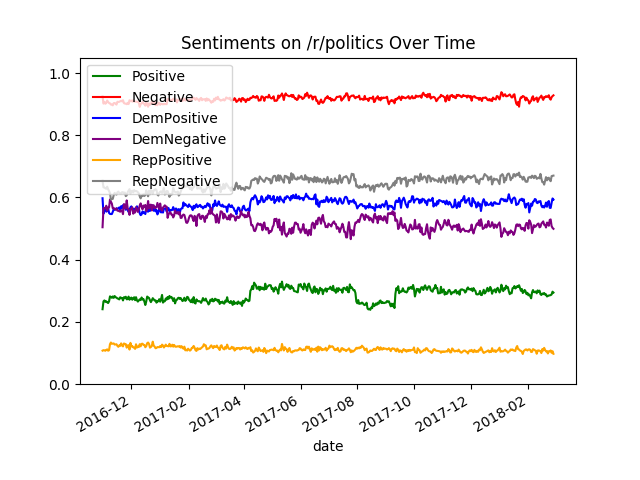
\includegraphics[height=3.5in]{plot1_sentiment_over_time.png}
                \caption{Percentage of comments with a given sentiment by date.
                The positive and negative lines are for Trump. The remaining four
                are for Democrat and Republican.}
        \end{center}
\end{figure}

\section{Sentiment by Location}

\begin{figure}[H]
        \begin{center}
                \minipage{0.5\textwidth}
                          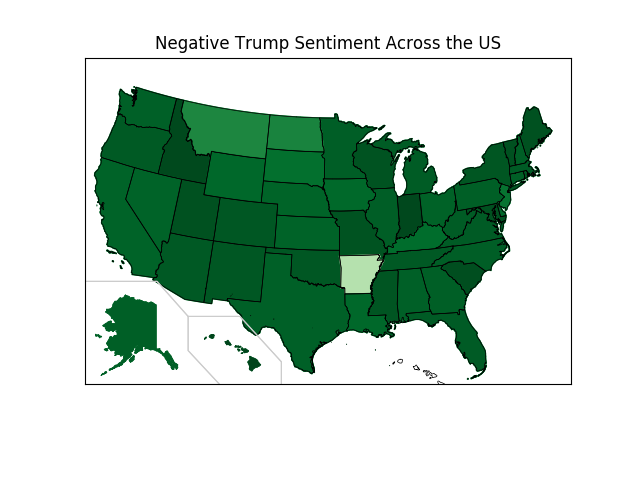
\includegraphics[width=\linewidth,trim={2cm 2cm 1.65cm 0},clip]{plot2_negative_by_state.png}
                \endminipage\hfill
                \minipage{0.5\textwidth}
                          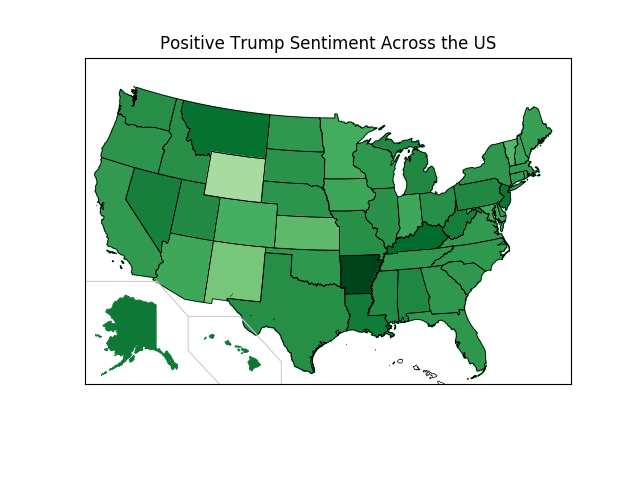
\includegraphics[width=\linewidth,trim={2cm 2cm 1.65cm 0},clip]{plot2_positive_by_state.png}
                \endminipage\hfill
                \minipage{0.8\textwidth}
                          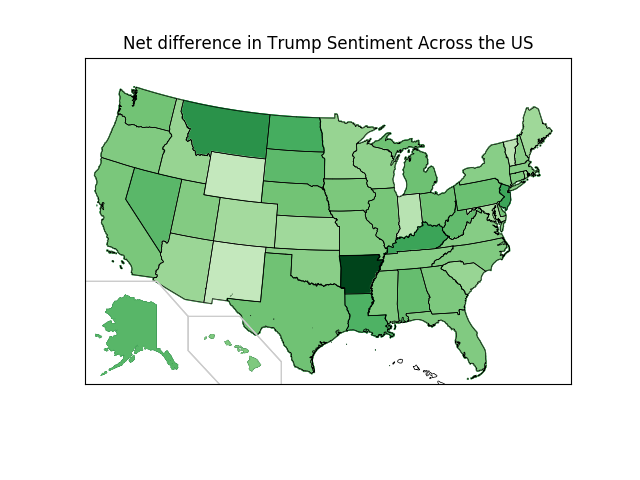
\includegraphics[width=\linewidth,trim={2cm 2cm 1.65cm 0},clip]{plot3_difference_by_state.png}
                \endminipage
        \end{center}
        \caption{Heat map of Trump sentiment. Darker colors indicate a higher percentage of comments with a given sentiment.}
\end{figure}

\section{Top 10 Submissions}

\subsection{Top 10 Positive Trump Submissions}

{\scriptsize
\begin{enumerate}
        \item Happy Election Day
        \item A New Subreddit for Serious Only Discussion of the Trump Presidency---No Memes, No Pepe's, Just Serious Discussion
        \item Assange denies backing Trump, liking either candidate
        \item Just told my mom im not voting for Hillary Clinton and this happened
        \item Kurt Eichenwald's Tweets Listing His Findings From His Newsweek Trump Investigation
        \item Historic Mississippi black church burned and vandalized with `Vote Trump' graffiti
        \item We should start a campaign to free Donalds Twitter account
        \item Trump \& Brexit International Coverage Bias
        \item Clinton has the edge one day before election
        \item Why would investing in gold and BTC be profitable because Trump won?? What does Trump being president have anything to do with gold and BTC?
\end{enumerate}
}

\subsection{Top 10 Negative Trump Submissions}

{\scriptsize
\begin{enumerate}
        \item Meet the unopposed Assembly candidate who says climate change is a good thing that hurts `enemies on the equator'
        \item U.S. Supreme Court Allows Arizona To Enforce Ban On Ballot-Collecting
        \item Bill Weld on Rachel Maddow: `I'm Here Vouching for Mrs. Clinton'
        \item Just told my mom im not voting for Hillary Clinton and this happened
        \item Election maps are telling you big lies about small things
        \item Hillary Clinton's challenge: Shift focus back to Trump
        \item There was no gun!
        \item Racism Alone Doesn't Explain Trump's Support, Which Also Reflects Economic Anxiety
        \item U.S. House Speaker Ryan renews call to suspend classified briefings for Clinton
        \item Investigating Donald Trump, F.B.I. Sees No Clear Link to Russia
\end{enumerate}
}

\subsection{Top 10 Positive Democrat Submissions}
{\scriptsize
\begin{enumerate}
        \item James Comey's casting of innuendo reminiscent of J. Edgar Hoover
        \item \#nonpartisan \#thissucks \#wawa
        \item Meet the unopposed Assembly candidate who says climate change is a good thing that hurts `enemies on the equator'
        \item Investigating Donald Trump, F.B.I. Sees No Clear Link to Russia
        \item In Colorado, gap between Democratic and Republican strategies is clear
        \item Republican activists to monitor Election Day polls
        \item U.S. Supreme Court Allows Arizona To Enforce Ban On Ballot-Collecting
        \item Report: Trump used dubious tax avoidance scheme in 1990s
        \item F.B.I. Says It Hasn't Changed Its Conclusions on Hillary Clinton Email Case
        \item Election maps are telling you big lies about small things
\end{enumerate}
}

\subsection{Top 10 Negative Democrat Submissions}

{\scriptsize
\begin{enumerate}
        \item The Top Democrat in the Country is a Neoliberal Disaster
        \item Lena Dunham just left Speaker Paul Ryan (R-WI) a voicemail. Here's what she said
        \item Obama promises smooth transition to Trump: `We are all rooting for his success'
        \item Meet the unopposed Assembly candidate who says climate change is a good thing that hurts `enemies on the equator'
        \item Famous personalities react to Donald Trump's electoral win
        \item Report: Trump used dubious tax avoidance scheme in 1990s
        \item Clinton versus the Turnip
        \item Keith Ellison laughed at for suggesting Trump could be GOP's nominee
        \item Historic Mississippi black church burned and vandalized with `Vote Trump' graffiti
        \item Bare-chested protesters removed from Trump's polling site
\end{enumerate}
}

\subsection{Top 10 Positive Republican Submissions}

{\scriptsize
\begin{enumerate}
        \item Obama To End Automatic Residency For Cuban Migrants
        \item Lawmakers Call For Probe Into Flynn's Russian Communications
        \item Canada PM Trudeau, Trump discuss border cooperation, lumber
        \item Trump is bad, Hillary is good
        \item Medical Debt Is Top Reason Consumers Hear From Collection Agencies
        \item Immigration ban includes green card holders: DHS
        \item Paul Ryan refuses to say whether health bill would pass House if vote were Wednesday
        \item Lithuania Braces for Putin ... and Trump
        \item House passes bill to curb class action lawsuits
        \item President Trump, does your daughter's new job in the White House fall in line with ethics guidelines?
\end{enumerate}
}

\subsection{Top 10 Negative Republican Submissions}

{\scriptsize
\begin{enumerate}
        \item There was no gun!
        \item Clinton has the edge one day before election
        \item U.S. Supreme Court Allows Arizona To Enforce Ban On Ballot-Collecting
        \item Election maps are telling you big lies about small things
        \item F.B.I. Says It Hasn't Changed Its Conclusions on Hillary Clinton Email Case
        \item Republican activists to monitor Election Day polls
        \item Top Democrats say Clinton took a real hit from Comey. But they're cautiously optimistic.
        \item Investigating Donald Trump, F.B.I. Sees No Clear Link to Russia
        \item \#nonpartisan \#thissucks \#wawa
        \item Janet Reno, First Woman to Serve as U.S. Attorney General, Dies at 78
\end{enumerate}
}

\section{Sentiment by Submission Score and Comment Score}

\begin{figure}[H]
        \minipage{0.5\textwidth}
                  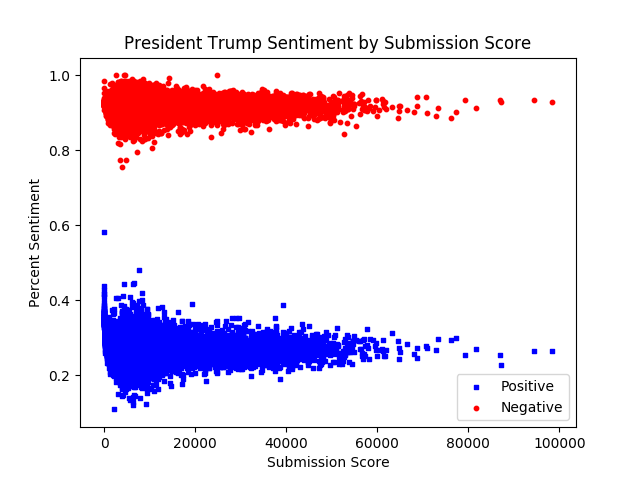
\includegraphics[width=\linewidth]{plot5a_djt_sentiment_by_story.png}
        \endminipage\hfill
        \minipage{0.5\textwidth}
                  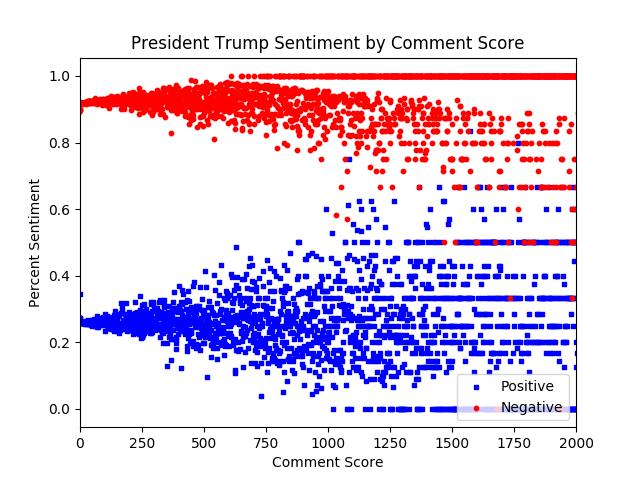
\includegraphics[width=\linewidth]{plot5b_djt_sentiment_by_comment.png}
        \endminipage
        \caption{Trump sentiment by submission and comment score.}
\end{figure}

\begin{figure}[H]
        \minipage{0.5\textwidth}
                  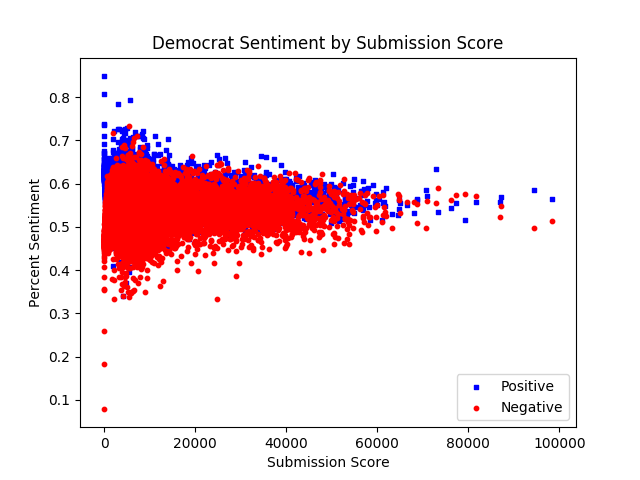
\includegraphics[width=\linewidth]{plot5a_dem_sentiment_by_story.png}
        \endminipage\hfill
        \minipage{0.5\textwidth}
                  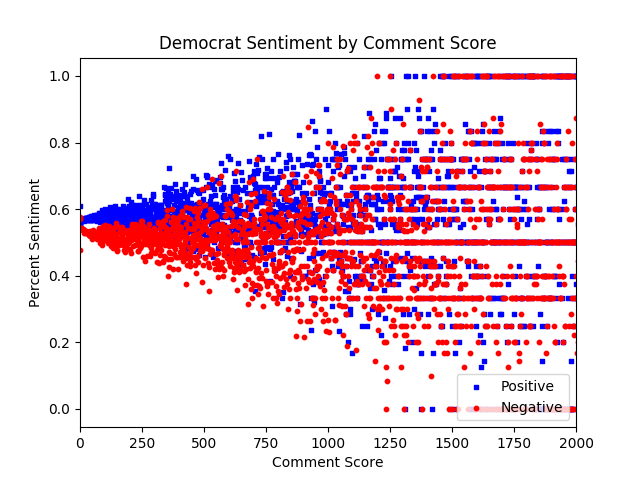
\includegraphics[width=\linewidth]{plot5b_dem_sentiment_by_comment.png}
        \endminipage
        \caption{Democrat sentiment by submission and comment score.}
\end{figure}

\begin{figure}[H]
        \minipage{0.5\textwidth}
                  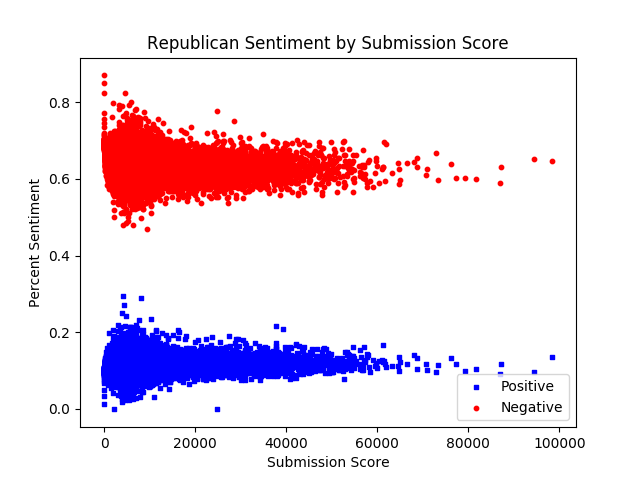
\includegraphics[width=\linewidth]{plot5a_rep_sentiment_by_story.png}
        \endminipage\hfill
        \minipage{0.5\textwidth}
                  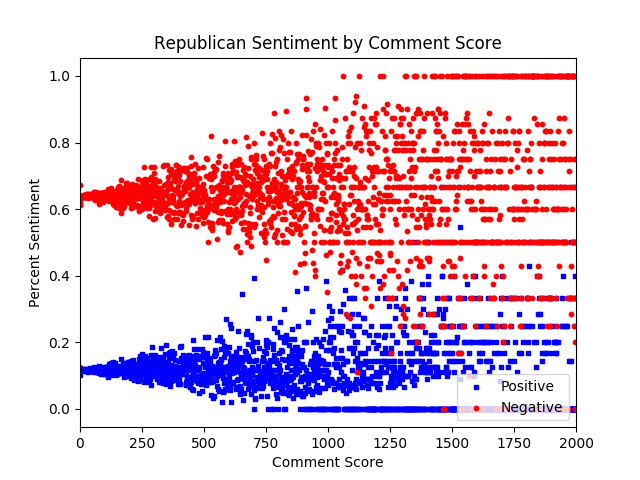
\includegraphics[width=\linewidth]{plot5b_rep_sentiment_by_comment.png}
        \endminipage
        \caption{Republican sentiment by submission and comment score.}
\end{figure}

\section{ROC Curves}

\begin{figure}[H]
        \minipage{0.5\textwidth}
                  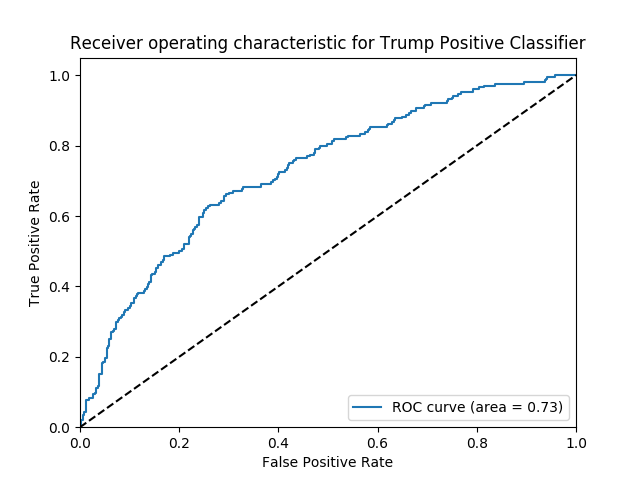
\includegraphics[width=\linewidth]{TrumpPositiveClassifier.png}
        \endminipage\hfill
        \minipage{0.5\textwidth}
                  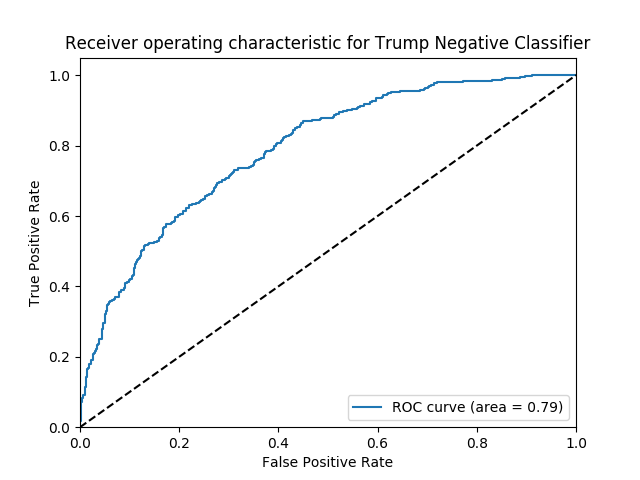
\includegraphics[width=\linewidth]{TrumpNegativeClassifier.png}
        \endminipage
        \caption{ROC curves for our Trump classifiers.}
\end{figure}

\begin{figure}[H]
        \minipage{0.5\textwidth}
                  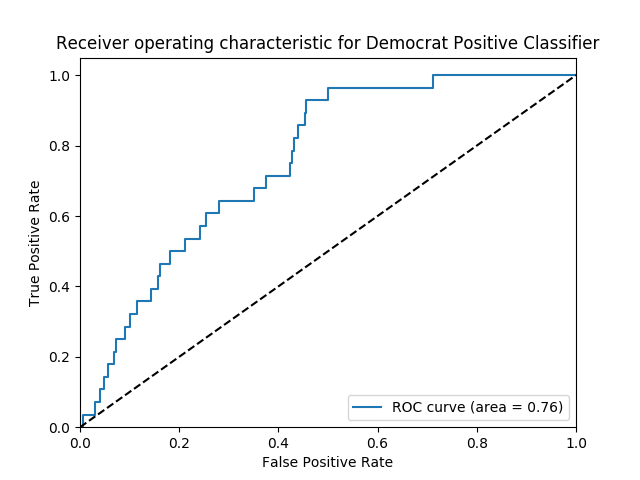
\includegraphics[width=\linewidth]{DemocratPositiveClassifier.png}
        \endminipage\hfill
        \minipage{0.5\textwidth}
                  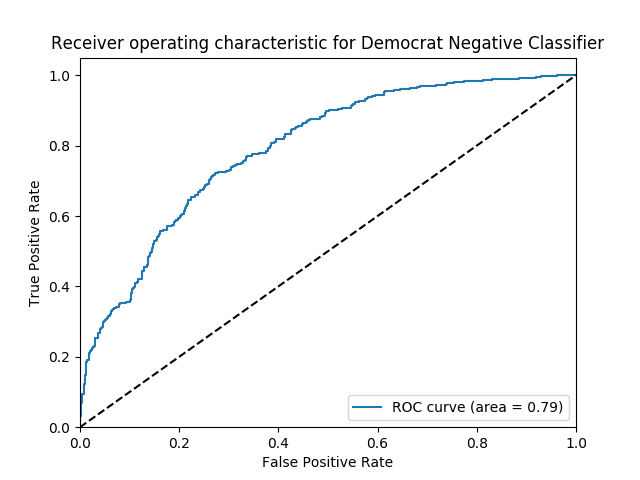
\includegraphics[width=\linewidth]{DemocratNegativeClassifier.png}
        \endminipage
        \caption{ROC curves for our Democrat classifiers.}
\end{figure}

\begin{figure}[H]
        \minipage{0.5\textwidth}
                  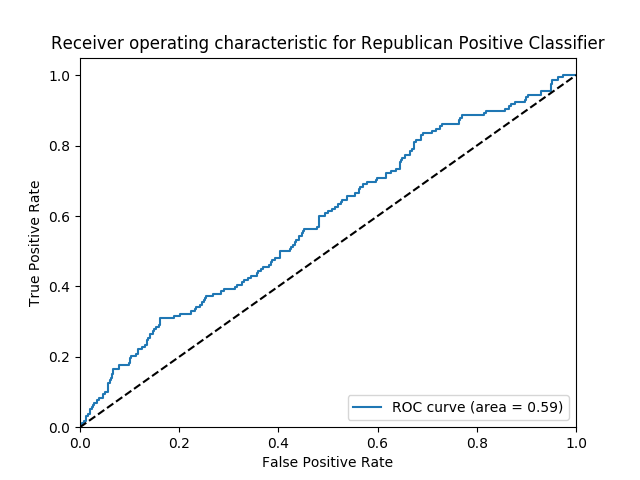
\includegraphics[width=\linewidth]{RepublicanPositiveClassifier.png}
        \endminipage\hfill
        \minipage{0.5\textwidth}
                  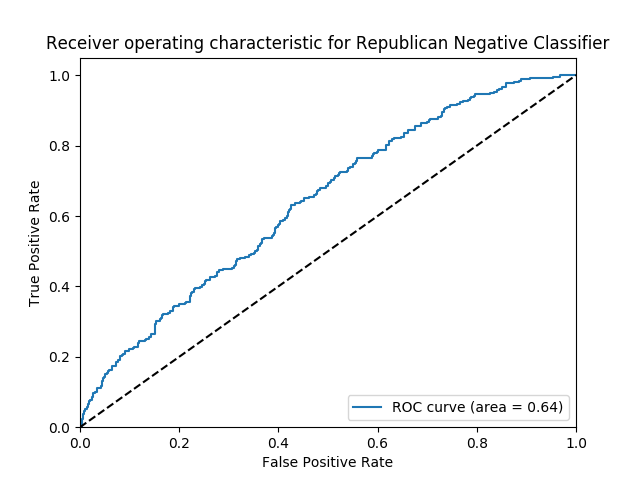
\includegraphics[width=\linewidth]{RepublicanNegativeClassifier.png}
        \endminipage
        \caption{ROC curves for our Republican classifiers.}
\end{figure}

\section{Summary}

\subsection{Trump}

Based on our generated heat maps, there tends to be fairly strong negative sentiment against President
Trump across all states except Arkansas, which has significantly weaker negative sentiment.
There appears to be mild to medium positive sentiment across the nation toward President
Trump. Most states are almost the same color with the exception of Wyoming and Arkansas. Wyoming has a
significantly smaller degree of positive sentiment and Arkansas has a noticeably stronger degree of positive
sentiment compared to other states. Other than these two states, there is only slight variation in sentiment.
The Net Difference of Trump Sentiment heat map highlights this similarity in sentiment.

For the top 10 stories, it’s clear that ``Happy Election Day'' is a pro-Trump story because it is celebrating
his victory. The top anti-Trump story calls Trump out for not supporting climate change.

The negative sentiment towards Trump is relatively consistent over time. However, positive sentiment on Trump jumps slightly
from April 2017 to August 2017 and again after September 2017. These time periods correspond to his election campaign.
With respect to submission scores, positive Trump sentiment was generally low at around 20\%-40\% while negative
Trump sentiment was much higher at around 80\%-100\%. The same trend carried true for comment score, in which
positive Trump sentiment centered a little below 20\% and negative Trump sentiment centered around 60\%.
Surprisingly, a better score did not correlative either a more positive or negative sentiment.

\subsection{Republican and Democrat}

It appears that Democrat sentiment is extremely conflicted between positive and negative with regard to submission score.
Both positive and negative Democrat sentiments center around 50\% with a spread of approximately 20\% regardless of submission score.
Republican sentiment is much more polarized with respect to submission score. Positive Republican sentiment centered around 0\%-20\%
while negative Republican sentiment centered around 60\%-80\% regardless of submission scores. As submission score increases,
the average sentiment percentage does not change but the spread tends to decrease significantly.

Democrat and Republican sentiment with respect to comment score observes similar values of average positive and negative
sentiment. But rather than decreasing spread as submission scores do, spread tends to increase as comment score increases.
Our figure shows spread increasing from less than 10\% to more than 30\% for each sentiment classifier.

Over time, we observe the same trend as we observed with Republican and Democratic sentiments as we observed with Trump, though to a
lesser degree. For instance, Democratic positive sentiment jumped from April 2017 to August 2017 as Democratic negative sentiment
decreased during the same time frame.

Overall the Democrat and Republican sentiment data did not provide very useful information. This may be due to poorly labeled data
that was provided to us or a training size that was too small.

\subsection{ROC Curves}

Our AUROC value for positive Trump sentiment was .73 while our AUROC value for negative Trump sentiment was .79.
We are satisfied with our AUROC value because it is close to what Professor Rosario achieved with his classifier.

Furthermore, for our Democrat Negative Classifier our AUROC value was .79 while our ROC curve value for Democrat
Positive Classifier was .76. We are also satisfied with this classifier's scores. However, the Democrat Positive
Classifier was only able to train and test with about 50 positive examples, which is why the ROC curve is very jagged.
This may not be enough data to get a good classifier.

In addition, our ROC area values for Republican positive sentiment for positive was .59, and our ROC curve value
for Republican negative sentiment for negative was .64. This shows that our model is currently not very accurate
in classifying Republican sentiment.

On a more general note, we understand that having a AUROC value closer to 1 will be
more beneficial because we have more discriminatory power between true and false positives. A good
classifier will have a high AUROC score because it will predict most positive examples correctly while not predicting
many false positives.

\section{Questions}

\subsection{Functional Dependencies in \texttt{labeled\_data.csv}}

There will be 3 minimum functional dependencies as shown below.
\begin{align*}
        f = \{&\texttt{input\_id} \rightarrow \texttt{labeldem},\\
        &\texttt{input\_id} \rightarrow \texttt{labelgop},\\
        &\texttt{input\_id} \rightarrow \texttt{labeldjt}\}
\end{align*}
As a result, there will also be functional dependencies derived from this minimal set
based on the properties of functional dependencies, such as
\[\texttt{input\_id} \rightarrow (\texttt{labeldem}, \texttt{labelgop})\]
The closure will be
\[f^+ = \{\texttt{input\_id} \rightarrow (\texttt{labeldem}, \texttt{labelgop}, \texttt{labeldjt})\}\]

\subsection{Normalization of \texttt{labeled\_data.csv}}

The data does not appear to be normalized, since there are redundancies in the attributes
that may affect the insert update integrity. For example, there is a functional
dependency between the \texttt{subreddit} attribute and the \texttt{subreddit\_id} attribute.
However, the \texttt{subreddit\_id} attribute is not a superkey. Thus, this is redundant.

In order to decompose the data, we would separate out the \texttt{subreddit} and \texttt{subreddit\_id} into a new
table with \texttt{subreddit\_id} as the superkey and the \texttt{subreddit} as an attribute. Then, we would associate
the new table with the comments table by making the \texttt{subreddit\_id} attribute into a
foreign key.

Also, we would do the same thing with \texttt{author}, creating a separate table with \texttt{author} and \texttt{subreddit\_id}
as the superkey, having attributes of \texttt{author\_flair\_text}, \texttt{author\_flair\_css\_class}. These depend on both the
subreddit and the author.

Finally we would have a table with \texttt{author} as the superkey and \texttt{can\_gild} as an attribute, since this only
depends on the author.

In addition, we could remove a couple derived fields from the schema such as
removing \texttt{is\_submitter} and \texttt{author\_cakeday}. Because we do not want somebody who is not
the OP is inserted into the comments relation with \texttt{is\_submitter} being true, we remove the attribute to maintain the data
integrity of our relation. Similarly for \texttt{author\_cakeday}, we can compare a user's account creation date to the
comment date to generate this field.

The collector of the data most likely stored the data in this manner to make filtering and aggregations on
this data much more efficient. For example, we can obtain the OP's information checking to see if a comment has
\texttt{is\_submitter} being true and then pulling out \texttt{author}, \texttt{author\_cakeday}, etc.
This is more efficient than performing a join across tables to get author information.

\subsection{Spark Join Explanation}

The output of the \texttt{explain()} function for the join
\begin{center}
        \scriptsize\texttt{labelled\_comments = comments.join(labels, comments.id == labels.Input\_id)}
\end{center}
is shown below.
{\scriptsize
\begin{verbatim}
== Physical Plan ==
*(2) BroadcastHashJoin [id#14], [Input_id#170], Inner, BuildRight
:- *(2) Project [author#0, author_cakeday#1, author_flair_css_class#2,
author_flair_text#3, body#4, can_gild#5, can_mod_post#6, collapsed#7,
collapsed_reason#8, controversiality#9L, created_utc#10L, distinguished#11, edited#12,
gilded#13L, id#14, is_submitter#15, link_id#16, parent_id#17, permalink#18,
retrieved_on#19L, score#20L, stickied#21, subreddit#22, subreddit_id#23,
subreddit_type#24]
:  +- *(2) Filter isnotnull(id#14)
:     +- *(2) FileScan parquet [author#0,author_cakeday#1,author_flair_css_class#2,
author_flair_text#3,body#4,can_gild#5,can_mod_post#6,collapsed#7,collapsed_reason#8,
controversiality#9L,created_utc#10L,distinguished#11,edited#12,gilded#13L,id#14,
is_submitter#15,link_id#16,parent_id#17,permalink#18,retrieved_on#19L,score#20L,
stickied#21,subreddit#22,subreddit_id#23,subreddit_type#24]
Batched: true, Format: Parquet, Location:
InMemoryFileIndex[file:/media/sf_vm-shared/project2b/parquets/comments.parquet],
PartitionFilters: [], PushedFilters: [IsNotNull(id)], ReadSchema:
struct<author:string,author_cakeday:boolean,author_flair_css_class:string,
author_flair_text:strin...
+- BroadcastExchange HashedRelationBroadcastMode(List(input[0, string, true]))
   +- *(1) Project [Input_id#170, labeldem#171, labelgop#172, labeldjt#173]
        +- *(1) Filter isnotnull(Input_id#170)
        +- *(1) FileScan parquet [Input_id#170,labeldem#171,labelgop#172,labeldjt#173]
Batched: true, Format: Parquet,
Location: InMemoryFileIndex[file:/media/sf_vm-shared/project2b/parquets/labels.parquet],
PartitionFilters: [], PushedFilters: [IsNotNull(Input_id)],
ReadSchema: struct<Input_id:string,labeldem:string,labelgop:string,labeldjt:string>
\end{verbatim}
}

Spark is using the Broadcast Hash Join. This is Spark's version of a Hash Join which is used when the size of a
dataframe is below Spark's broadcast join threshold and can fit into memory. Since the size of the \texttt{labels}
dataframe contains only 2000 rows, it meets this criteria.

Spark seems to be using two worker nodes running in parallel to join the two dataframes. On one node 1,
Spark scans in the label parquet. Then, it filters out any rows with a null \texttt{Input\_id}. This should not change
the data because \texttt{Input\_id} is a candidate key for the table. So none of the rows in the table should
have a null \texttt{Input\_id}.

Next, Spark projects to obtain to obtain the columns \texttt{Input\_id}, \texttt{labeldem},
\texttt{labelgop}, and \texttt{labeldjt}. At this point, the worker node broadcast exchanges this result
to the other worker node 2. On the other worker node 2, Spark scans in the comments parquet. Then, it
filters for any null \texttt{id}'s. Again, this should not change the data because since \texttt{id} is a candidate key
for the table. Next, it projects to obtain to obtain all the columns in the table. Then, once it starts
receiving the exchange broadcast from the other worker node, Spark executes a Broadcast Hash Join to hash
join the results.

\end{document}